\documentclass[11pt,a4paper]{article}

\usepackage[utf8]{inputenc}
\usepackage[margin=1in]{geometry}
\usepackage{amsmath,amssymb}
\usepackage{graphicx}
\usepackage{booktabs}
\usepackage{tabularx}
\usepackage{hyperref}
\usepackage{caption}
\usepackage{subcaption}
\usepackage{float}
\usepackage{microtype}
\usepackage{enumitem}
\usepackage{xcolor}

\hypersetup{
    pdftitle={Changing Patterns of Occupation, Ecological Niches, and Socio-Economic Interdependence in Chamba District (1881-1961)},
    pdfauthor={Bala Subramanian, Vagdevi Reddy, Phanindra},
    colorlinks=true,
    linkcolor=blue!70!black,
    citecolor=blue!70!black,
    urlcolor=blue!70!black
}

\title{\Large\textbf{Changing Patterns of Occupation, Ecological Niches, and Socio-Economic Interdependence in Chamba District (1881--1961)}\\[0.4em]
\large A Computational and Historiographical Analysis of Himalayan Agrarian and Pastoral Systems}

\author{
    \textbf{Bala Subramanian} \and 
    \textbf{Vagdevi Reddy} \and 
    \textbf{Phanindra} \\[0.5em]
    \normalsize Course: Introduction to Historical Analysis
}
\date{}

\begin{document}

\maketitle

\noindent\textbf{Project Repository:} \url{https://github.com/phanindragollapalli/History_project}

\vspace{0.8em}

\begin{abstract}
This study investigates how changing patterns of occupation and economic interdependence shaped caste and religious relations in the upper Ravi River basin of Chamba District, Himachal Pradesh, between 1881 and 1961. Moving beyond colonial tropes of static, isolated mountain autarkies, we construct an epistemological dialogue between the deductive framework of Historical Materialism and the inductive method of the \textit{Annales} school of environmental history, deployed alongside computational text analysis across four benchmark periods: the 1881 Imperial Census (Ibbetson), the 1911--1919 Ethnographic Glossary (Rose), the 1931 Census (Khan), and three 1961 Village Surveys (Brahmaur, Chitrari, and Maingal). We demonstrate that social hierarchy, labour exploitation, and inter-community co-existence were grounded in the material organization of production operating across sharp altitudinal gradients. First, at the level of the \textit{longue dur\'ee}, environmental altitude imposed an absolute biological ceiling on animal husbandry: water buffaloes suffered severe cold-induced lactation collapse (dropping by 55.6\% from 9 to 4 seers per day) in alpine Brahmaur ($\sim$7,000 ft), permanently barring dairy transhumance into the highlands and securing the Gaddi monopoly over sheep pastoralism, while confining commercial buffalo dairying to sub-Himalayan Maingal ($\sim$4,000 ft). Second, at the conjunctural level of production relations, dominant proprietors who monopolized accumulated surplus (``dead labour'' in land and flocks) were structurally dependent on subordinate ``living labour'': Sipis in Brahmaur maintained an indispensable tripartite monopoly as contractual wage shepherds (\textit{pohals} receiving cash, wool, and a 2--4\% lamb dividend), master tweed weavers, and \textit{Nawala} ritual drummers; attached Halis in Chitrari tilled Brahmin lands to circumvent high-caste plough taboos while mobilizing under the Arya Samaj as \textit{Aryas--Halis}; and Lohar blacksmiths in Maingal were remunerated through customary unhusked grain sheaves (\textit{khalian}) from harvest threshing floors. Third, peaceful Hindu-Muslim co-existence in Maingal was sustained by complementary, non-competing ecological niches between Gujjar forest buffalo pastoralism and Brahmin terraced farming. Customary reciprocity did not vanish with market expansion; rather, cash contracts, in-kind barter, ritual perquisites, and commercial commodity sales operated concurrently as an integrated, multi-tiered economy.
\end{abstract}

\vspace{0.5em}
\noindent\textbf{Keywords:} Himalayan Agro-Pastoralism, Transhumance, Gaddis, Gujjars, Historical Materialism, Annales School, Longue Dur\'ee, Histoire Totale, Dead vs. Living Labour, Jajmani Barter, Computational History, Chamba State.

\newpage
\tableofcontents
\newpage

\section{Introduction and Historiographical Problem}

In nineteenth-century British colonial ethnography and settlement reports, mountain societies in the Western Himalayas were depicted as timeless isolates governed by archaic caste codes. From Denzil Ibbetson's census treatises to B. H. Baden-Powell's village studies, colonial archives framed Himalayan valleys as insular ``village republics'' where ancient Hindu social formations survived frozen in amber, isolated from external commercial networks and regional trade corridors. Subaltern mountain populations were reified into paternal, racialized taxonomies that classified hill communities into rigid occupational compartments, ignoring the dynamic negotiations of labour, seasonal mobility, and inter-community accommodations that sustained mountain life.

This essay challenges such static conceptions through an intensive micro-comparative and computational historical investigation of the upper Ravi River basin in Chamba District, Himachal Pradesh, spanning the late nineteenth century to 1961. Our central research question asks:
\begin{quote}
\textit{How did changing patterns of occupation and economic interdependence shape caste and religious relations in Brahmaur, Chitrari, and Maingal of Chamba district from the late nineteenth century to 1961?}
\end{quote}

Rather than treating rural Chamba as a uniform cultural landscape, our investigation compares three distinct settlements situated across sharp altitudinal and ecological gradients within the upper Ravi drainage:
\begin{enumerate}[leftmargin=*]
    \item \textbf{Brahmaur (Brahmaur Sub-Tehsil / Gaderan, $\sim$7,000 ft):} An alpine settlement centered on transhumant Gaddi sheep and goat pastoralism, seasonal migration across the glaciated passes of the Dhaula Dhar and Pir Panjal ranges, the sacred Chaurasi temple complex, and institutionalized service relations between upper-caste flock owners (Rajputs and Brahmans) and lower-caste artisan specialists (Sipis and Reharas).
    \item \textbf{Chitrari (Chamba Tehsil, $\sim$5,800 ft):} An intermediate terraced river basin dominated by landed Brahmin hegemony (comprising 77\% of the surveyed population) rooted in historic eighth-century royal land grants (\textit{shasan}) from Raja Meru-Varman to the Shakti Devi temple, intensive plough cultivation, attached ploughmen labour (\textit{Halis}), and seasonal dairy trade with nomadic pastoralists.
    \item \textbf{Maingal (Chamba Tehsil, $\sim$4,000 ft):} A sub-Himalayan forested slope presenting a multi-religious frontier where settled Muslim Gujjar buffalo pastoralists residing in dispersed forest \textit{kothas} (81.5\% of the population) co-existed, traded, and shared resources with nucleated settlements of Hindu Brahmins, Rajputs, and blacksmith artisans (\textit{Lohars}).
\end{enumerate}

Following the \textit{Annales} agenda of \textit{histoire-probl\`eme} and micro-history, we look intensively at these small units of space and time to answer broader questions regarding Himalayan agrarian and pastoral transitions. We argue that caste hierarchies, inter-community accommodations, and religious co-existence in the upper Ravi were shaped not by abstract scriptural dogmas, but by the material organization of work and exchange operating within strict ecological boundaries. Altitudinal relief established physiological ceilings that dictated viable productive regimes. These production systems generated dense webs of mutual dependence between landed proprietors, mobile graziers, craft specialists, and menial workers. Crucially, the expansion of monetary trade did not displace customary relations in a linear transition to market capitalism. Instead, cash wages, tied crop shares, unhusked grain perquisites, ritual meat entitlements, and commercial bazaar sales functioned concurrently as a multi-tiered economy. Social status was thus continuously reproduced, negotiated, and contested within locally specific agrarian and pastoral systems conditioned by mountain ecology and filtered through shifting colonial classification schemes.

The remainder of this essay is structured as follows: Section 2 outlines our theoretical framework, synthesizing Historical Materialism with the \textit{Annales} school. Section 3 details the four-tiered archive and computational pipeline. Section 4 examines how altitudinal gradients established biological ceilings on animal husbandry. Section 5 evaluates the micro-organization of labour, caste asymmetries, and the 12-relationship exchange network. Section 6 investigates inter-religious co-existence, market mobility, material culture, and vernacular oral ballads. Section 7 traces longitudinal classification drift from 1881 to 1961. Section 8 synthesizes our findings and wider historiographical significance.

\section{Historiographical and Theoretical Framework}

To analyze the relationship between physical environment, labour organization, and social hierarchy across our archival corpus, we construct a methodological framework synthesizing Historical Materialism with the \textit{Annales} school of social and environmental history.

\subsection{The Epistemological Dialogue: Deductive Theory and Inductive Method}
Historical analysis navigates between two foundational epistemological orientations: the deductive and the inductive. Historical Materialism operates primarily as a deductive theory of historical development, positing that the material conditions of production constitute the foundational infrastructure of human society, from which social structures, political institutions, and ideological forms arise. Conversely, the \textit{Annales} school, founded by Marc Bloch and Lucien Febvre in 1929, proceeds from an inductive foundation: it rejects grand \textit{a priori} schemas, insisting on the meticulous gathering, collation, and statistical analysis of empirical facts across the full spectrum of human and environmental experience to construct historical explanations.

Rather than treating these traditions as mutually exclusive, our study synthesizes their analytical strengths. The inductive method of the \textit{Annales} school guides our empirical and computational handling of archival sources, gathering multi-temporal census statistics, constructing longitudinal concordance indices, and recovering the material realities of everyday life. Meanwhile, the deductive insights of Historical Materialism provide the theoretical categories necessary to interpret those empirical patterns, uncovering how ownership of productive assets, the extraction of surplus, and the structural contradictions of class and caste generated specific forms of social interdependence.

\subsection{Historical Materialism: Labour, Dead Surplus, and Relations of Production}
A rigorous Marxist analysis begins with the materialist premise: ``matter is primary, idea is secondary.'' As Friedrich Engels articulated in \textit{The Origin of the Family, Private Property and the State}, the determining factor in history is, in the final instance, the production and reproduction of immediate life. This fundamental process possesses a twofold character: the production of the means of existence (food, clothing, shelter, and tools), and the biological propagation of the species.

In the agrarian and pastoral ecology of the Western Himalayas, this materialist conception illuminates several critical dynamics:
\begin{itemize}[leftmargin=*]
    \item \textbf{Labour as Conscious Human Action:} Labour distinguishes human beings from the natural world. As Engels observed, ``the hand is not only the organ of labour, it is also the product of labour.'' In mountain terrain, human survival is the direct outcome of conscious, planned physical labour applied to harsh natural conditions, terracing steep hillsides, engineering gravity irrigation channels (\textit{kuhls}), spinning fleece, and driving herds across glaciated alpine cols.
    \item \textbf{Accumulated Surplus as ``Dead Labour'':} Social stratification arises when the division of labour generates an economic surplus beyond immediate biological subsistence. In Marxist terminology, accumulated surplus constitutes \textbf{dead labour}-past human labour crystallized into durable productive assets, specifically arable land titles, water mills, iron forge equipment, and transhumant livestock herds. Society is fundamentally divided between those who control accumulated dead labour (the proprietary classes) and those who possess only their \textbf{living labour} (their immediate capacity to work).
    \item \textbf{The Conflict and Unity of Opposites:} In rural Chamba, this structural division followed sharp caste fault lines. High-caste Rajputs and Brahmins held monopoly ownership over terraced land and transhumant flocks (controlling 97.9\% of all sheep and goats in Brahmaur). Lower-caste groups (Sipis, Halis, Lohars) owned minimal land and negligible herds. Yet, in accordance with the dialectical law of the unity and conflict of opposites, these classes were bound in structural interdependence. High-caste Brahmins in Chitrari, constrained by religious taboos prohibiting them from gripping the wooden plough, were paralyzed without the living labour of attached Halis. Rajput flock masters in Brahmaur could not shear wool, weave protective tweed, or undertake treacherous pass crossings without Sipi shepherds and weavers. Property ownership gave elites the power of surplus extraction, but their material survival depended on the technical labour of subordinate castes.
    \item \textbf{Base and Superstructure without Reductionism:} The material forces and social relations of production formed the economic base of Himalayan society. Legal customs, religious rituals, and caste purity ideologies constituted the superstructure that stabilized this base. Avoiding crude economic determinism, we recognize that the superstructure exercised reciprocal agency. Ritual ceremonies, such as the Shaivite \textit{Nawala} feast in Brahmaur, did not merely mask exploitation; they functioned as vital arenas of customary redistribution where lower-caste musicians received consecrated meat entitlements (\textit{ghardi}) and reasserted their ritual indispensability.
\end{itemize}

\subsection{The Annales School: Longue Dur\'ee, Histoire Totale, and Temporal Rhythms}
Complementing Historical Materialism, the \textit{Annales} school directs historical inquiry toward the physical environment and the slowly changing structures of daily existence. Rejecting traditional Rankean political history, the \textit{Annales} historians championed \textbf{Total History} (\textit{histoire totale})-the comprehensive study of all aspects of past human life: shelters, diet, clothing, production techniques, and human interaction with the non-human natural environment.

Central to this paradigm is Fernand Braudel's three distinct rhythms of historical time:
\begin{enumerate}[leftmargin=*]
    \item \textbf{Geographical Time (The \textit{Longue Dur\'ee}):} The time of physical structures, climate, geological relief, and biological adaptation. Stretching across centuries, changes in the \textit{longue dur\'ee} are imperceptible yet stable, providing the physical foundation within which human history unfolds. In the upper Ravi, the steep altitudinal zonation of the Dhaula Dhar and Pir Panjal ranges, lapse rates, and biological limits on livestock species constitute an enduring \textit{longue dur\'ee} dictating human possibilities.
    \item \textbf{Social-Economic Time (The Time of Conjuncture):} The medium-term rhythms of economic cycles, demographic trends, occupational structures, and agrarian systems spanning decades or a century. In our study, this conjuncture is traced across the eighty-year window from 1881 to 1961, encompassing the resilience of customary jajmani barter, the Great Depression's disruption of agrarian prices, and the gradual integration of mountain dairy and wool into regional cash markets.
    \item \textbf{Political and Event Time (\textit{L'Histoire \'Ev\'enementielle}):} The rapid, surface time of political events, administrative decrees, and short-term policies. In colonial Chamba, this level encompasses specific imperial decennial censuses, British settlement reports, and post-colonial statutory orders (such as the 1956 Scheduled Castes and Scheduled Tribes Orders). As Braudel insisted, political events make historical sense only when grounded in underlying structural rhythms.
\end{enumerate}

Furthermore, the \textit{Annales} tradition pioneered the \textbf{History of Mentalities} (\textit{histoire des mentalit\'es})-the study of collective psychological architectures, worldviews (\textit{Weltanschauung}), and emotional categories through which historical actors made sense of their existence. In our analysis, \textit{mentalit\'es} are recovered through the material culture of everyday life and the vernacular oral ballads of mountain shepherds and peasant women.

By integrating these theoretical paradigms, we establish an integrated analytical chain:
\begin{center}
\small
\fbox{\parbox{0.94\textwidth}{\centering
\textbf{Ecological Conditions (\textit{Longue Dur\'ee})} $\;\longrightarrow\;$ \textbf{Productive Strategies \& Asset Ownership (\textit{Base})}\\[0.3em]
$\;\longrightarrow\;$ \textbf{Division of Labour (Dead vs. Living Labour)} $\;\longrightarrow\;$ \textbf{Multi-Tiered Exchange Modes}\\[0.3em]
$\;\longrightarrow\;$ \textbf{Social Hierarchies, Mentalit\'es, and Status Contestation (\textit{Superstructure})}
}}
\end{center}

\section{Sources, Administrative Scale, and Computational Methodology}

Historical investigation in the Western Himalayas requires navigating disparate archival genres operating across a four-tiered administrative hierarchy:
\begin{center}
\small
\fbox{\parbox{0.94\textwidth}{\centering
\textbf{British Punjab Province} $\;\longrightarrow\;$ \textbf{Chamba Princely State} $\;\longrightarrow\;$ \textbf{Wazarats / Tehsils} $\;\longrightarrow\;$ \textbf{Villages / Hamlets}
}}
\end{center}

\subsection{The Archival Corpus across Four Benchmark Eras}
Our archival corpus covers four distinct chronological benchmarks spanning eighty years, combining macro-provincial demographic surveys with micro-household monographs (Table~\ref{tab:sources}).

\begin{table}[htbp]
\centering
\small
\caption{Primary Archival Source Corpus and Administrative Resolution}
\label{tab:sources}
\begin{tabularx}{\textwidth}{llcp{3cm}X}
\toprule
\textbf{Source Tag} & \textbf{Historical Era} & \textbf{Year} & \textbf{Administrative Scale} & \textbf{Analytical Focus and Character} \\
\midrule
Census 1881 & Early Colonial & 1881 & Punjab Province / Chamba State & Denzil Ibbetson; paternal colonial taxonomy; bi-regional land tenure across Dhaula Dhar (6 volumes; 696,820 words). \\
Rose Glossary & Late Colonial & 1911--19 & Punjab Hill States Agency & H. A. Rose; 4-tier Gaddi racial taxonomy; anti-pastoral revenue stereotypes; compilation based on 1881/1891 censuses (3 volumes; 789,702 words). \\
Census 1931 & Interwar Depression & 1931 & Punjab States / Chamba State & Khan Ahmad Hasan Khan; macro-demographic baseline; tripartite economic dependency shift (Earners/Dependents; 2 volumes; 338,055 words). \\
Brahmaur 1961 & Post-Independence & 1961 & Village Monograph No. 5 & Micro-census of 99 surveyed households (721 pop); 4,484 sheep/goats, 0 buffaloes; Sipi labour contracts; \textit{Nawala} ritual. \\
Chitrari 1961 & Post-Independence & 1961 & Village Monograph No. 10 & Micro-census of 79 surveyed households (404 pop); 77\% Brahmin majority; attached Halis (\textit{Aryas}); temple economy. \\
Maingal 1961 & Post-Independence & 1961 & Village Monograph No. 27 & Micro-census of 40 surveyed households (249 pop in 13 hamlets); 217 water buffaloes; Muslim Gujjar dairy economy; Lohar barter. \\
\bottomrule
\end{tabularx}
\end{table}

The 1881 Census (Ibbetson) mapped caste and tribal identities onto a functional taxonomy while documenting Gaddi bi-regional tenure across the Dhaula Dhar (summer grazing dues to Chamba, winter revenue to Kangra). Rose's Glossary (1911--1919) formalized a four-tier racialized Gaddi hierarchy while displaying anti-pastoral revenue bias. The 1931 Census (Khan) shifted to economic dependency categories (Principal Earners, Working Dependents) under Great Depression pressures. Finally, the 1961 Village Monographs provide granular micro-surveys of household budgets, livestock, caste divisions, and material culture in Brahmaur, Chitrari, and Maingal.

\subsection{Computational Pipeline Architecture}
To process this bilingual (English and Devanagari) archival corpus with algorithmic consistency, we developed an end-to-end Python pipeline rooted in the \textit{Annales} principles of serial and quantitative history:
\begin{enumerate}[leftmargin=*]
    \item \textbf{OCR Digitization and Preprocessing:} Scanned PDF volumes were extracted and processed using Tesseract OCR configured with multi-language models (\texttt{-l eng+hin} and \texttt{-l eng+urd+hin}). Textual streams were cleaned by stripping headers, footers, and scanning artifacts, producing standardized UTF-8 text corpora.
    \item \textbf{Keyword-in-Context (KWIC) Text Mining:} Python regex routines harvested contextual concordance windows ($\pm 250$ characters) surrounding all target community names (Gaddi, Gujjar, Sipi, Hali, Lohar, Brahmin, Rajput, Arya), economic terms (wage, grain, sheep, buffalo, plough, khalian), and institutions (temple, dhar, kotha). This generated 718 verified concordance extracts for 1881, 387 for Rose (1911--1919), 560 for 1931, and 1,038 for 1961.
    \item \textbf{Normalized Frequency Computation:} Because monograph lengths varied substantially (Brahmaur: 65,302 words; Chitrari: 41,363 words; Maingal: 70,551 words; 1881 Census: 696,820 words), raw keyword hit counts introduce severe distortions. We calculated normalized relative frequencies per 1,000 searchable words:
    \[
    \text{Normalized Relative Frequency} = \left( \frac{\text{Absolute Keyword Hits}}{\text{Total Searchable Words in Monograph}} \right) \times 1,000
    \]
    This metric measures \textit{textual salience} and administrative attention, rather than direct demographic proportion.
    \item \textbf{Thematic Multi-Label Qualitative Coding:} Using a structured protocol, 20 critical evidentiary passages (PAS\_001 to PAS\_020) were audited and coded across 9 themes: Labour Hierarchy (\texttt{LAB}), Economic Dependence (\texttt{DEP}), Exchange Modes (\texttt{EXC}), Ecology (\texttt{ECO}), Mobility (\texttt{MOB}), Religious Relations (\texttt{REL}), Gender (\texttt{GEN}), Ritual Economy (\texttt{RIT}), and Status Contestation (\texttt{POW}).
\end{enumerate}

\subsection{Archival Biases, Colonial Geo-Fixing, and Methodological Caveats}
A critical historical analysis must interrogate the epistemological distortions embedded within colonial and official archives:
\begin{itemize}[leftmargin=*]
    \item \textbf{Colonial ``Geo-Fixing'' vs. Mobile Reality:} As demonstrated in Annales environmental studies, colonial states sought to ``geo-fix'' fluid landscapes and mobile populations to render them taxable and predictable. Just as British engineers constructed embankments to confine meandering Gangetic rivers into static map coordinates, colonial census administrators attempted to fix transhumant pastoralists into static village boundaries. The seasonal movement of Gaddis and Gujjars was viewed by revenue officials as an administrative anomaly, generating hostile colonial stereotypes (e.g., Rose describing Gujjars as ``lazy cultivators fond of other people's cattle'').
    \item \textbf{The ``Absence Fallacy'':} Algorithmic keyword extraction must not confuse textual absence with historical non-existence. The absence of the word \textit{Gujjar} in the Brahmaur village survey does not mean nomadic pastoralists were absent from the upper district; rather, it reflects localized migratory corridors and the monograph's administrative scope.
    \item \textbf{Winter Census Seasonality:} The 1881 and 1931 imperial censuses were executed synchronously in mid-February, when alpine snows force transhumant Gaddis and Gujjars down into the lower foothills of Kangra, Gurdaspur, and Jammu. Consequently, highland censuses routinely undercounted pastoral populations and their livestock, misrepresenting them as sedentary farmers.
    \item \textbf{Administrative Scale Incommensurability:} Macro-provincial returns for Chamba State (e.g., 146,870 rural inhabitants in 1931) cannot be mathematically disaggregated to reconstruct the micro-demography of specific hamlets prior to the 1961 surveys. Computational comparisons across eras must focus on relational structures rather than continuous time-series statistics.
\end{itemize}

\section{Altitudinal Gradients and Ecological Niches}

The historical evolution of human settlement, agrarian technology, and social stratification in Chamba District was anchored in the physical topography of the Ravi River basin. Elevation above sea level governed ambient temperature, duration of snow cover, arable terrace stability, and vegetative fodder, creating three distinct micro-ecological zones across our study villages (Table~\ref{tab:comp_economy}).

\begin{table}[htbp]
\centering
\small
\caption{Comparative Village Occupational and Economic Structure (1961)}
\label{tab:comp_economy}
\begin{tabularx}{\textwidth}{p{2.3cm}p{3.2cm}p{2.8cm}p{2.6cm}X}
\toprule
\textbf{Village \& Elevation} & \textbf{Demographic Profile} & \textbf{Livestock Profile} & \textbf{Specialized Castes} & \textbf{Primary Labour \& Exchange Modes} \\
\midrule
\textbf{Brahmaur}\newline ($\sim$7,000 ft;\newline Alpine Valley) & 721 pop / 99 hh\newline Rajputs: 293 (40.6\%)\newline Brahmans: 251 (34.8\%) & 4,484 Sheep/Goats\newline 123 Bulls / 116 Cows\newline \textbf{0 Water Buffaloes} & Sipis: 119 (16.5\%)\newline Reharas: 22 (3.1\%)\newline Khatris: 28 (3.9\%) & Contractual wage shepherding (Rs.~2/mo + 2--4\% lamb shares); raw wool shares for weaving; sacrificial meat entitlements (\textit{ghardi}) for ritual drumming. \\
\midrule
\textbf{Chitrari}\newline ($\sim$5,800 ft;\newline Terraced Basin) & 404 pop / 79 hh\newline Brahmins: 311 (77.0\%)\newline Rathis: 32 (7.9\%) & 155 Oxen (ploughing)\newline 123 Sheep / 36 Goats\newline \textbf{0 Water Buffaloes} & Halis: 6 (1.5\%)\newline Bensis: 29 (7.2\%)\newline Rathis: 32 (7.9\%) & Attached tenancy ploughing for Brahmins; customary temple grain collections for Bensis; cash/cereal purchase of monsoon Gujjar milk. \\
\midrule
\textbf{Maingal}\newline ($\sim$4,000 ft;\newline Forest Slopes) & 249 pop / 40 hh\newline Muslim Gujjars: 203 (81.5\%)\newline Brahmins: 34 (13.7\%) & \textbf{217 Water Buffaloes}\newline 85 Cattle / Bullocks\newline 21 Sheep / Goats & Lohars: 8 (3.2\%)\newline Brahmins: 34 (13.7\%)\newline Rajputs: 4 (1.6\%) & Non-monetary threshing grain (\textit{khalian}) for ironwork; cash sale of commercial ghee in Chamba bazaar; reciprocal dung/bullock exchange. \\
\bottomrule
\end{tabularx}
\end{table}

\begin{figure}[htbp]
\centering
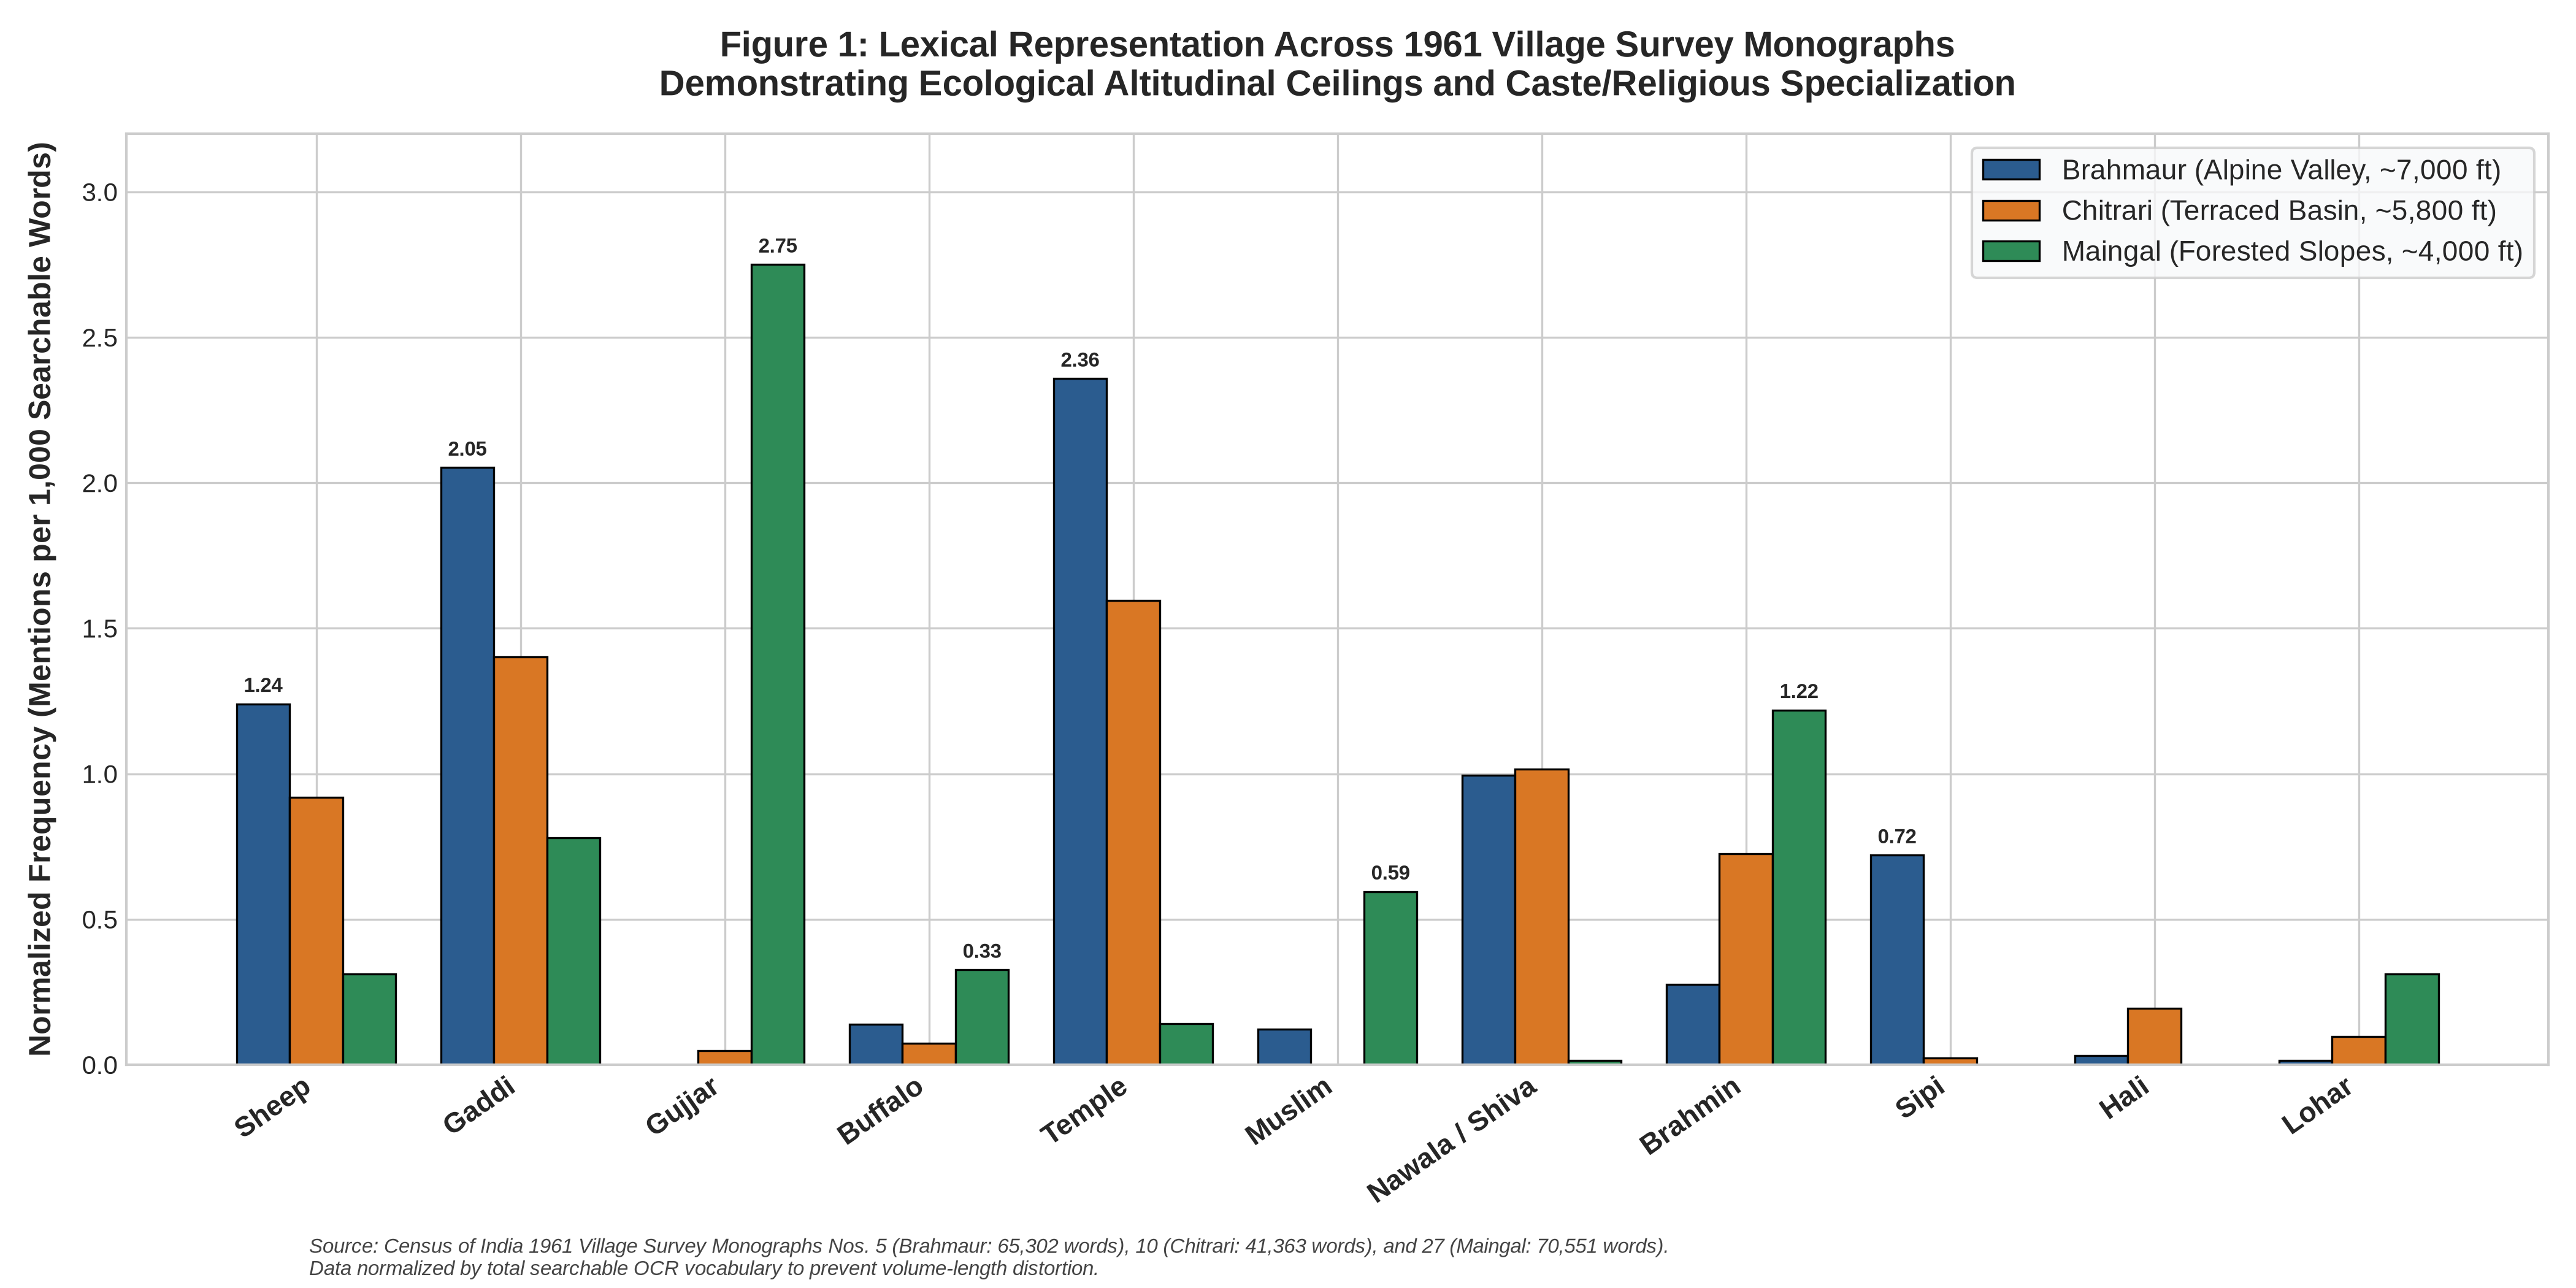
\includegraphics[width=0.92\textwidth]{outputs/figures/fig1_1961_village_mentions_normalized.png}
\caption{Normalized Relative Word Frequencies across 1961 Village Monographs (Mentions per 1,000 Words). Note the stark divergence: sheep, Gaddi, and temples dominate alpine Brahmaur; land, temples, and Brahmins peak in terraced Chitrari; Gujjars, buffaloes, and Lohars dominate forested Maingal.}
\label{fig:frequencies}
\end{figure}

The lexical frequency distributions plotted in Figure~\ref{fig:frequencies} visually confirm how administrative and communal focus reflected local ecological reality. In Brahmaur, textual prominence is monopolized by terms associated with pastoralism and religious ritual: \textit{sheep} (1.24 per 1,000 words), \textit{Gaddi} (3.63), and \textit{temple} (3.26). In Chitrari, the vocabulary centers on landed property and Brahminical authority: \textit{land} (2.61), \textit{Brahmin} (1.98), and \textit{temple} (2.85). In Maingal, the administrative text shifts entirely to pastoral dairying and artisanal service: \textit{Gujjar} (3.73), \textit{buffalo} (0.35), and \textit{Lohar} (0.16). These quantitative textual divergences mirror the underlying material structures of production.

\subsection{The Biological Ceiling on Pastoral Husbandry: A Longue Dur\'ee Constraint}
Nowhere is the explanatory power of environmental history clearer than in the distribution of livestock species across elevations (Figure~\ref{fig:livestock}).
\begin{itemize}[leftmargin=*]
    \item \textbf{Empirical Observation:} In high-altitude Brahmaur ($\sim$7,000 ft), sheep and goat pastoralism was the predominant form of wealth, with 4,484 animals enumerated across 48 pastoral households. In contrast, there were \textbf{precisely zero water buffaloes}. Conversely, in low-altitude Maingal ($\sim$4,000 ft), water buffaloes formed the core of the economy, totaling 217 head across 25 households (averaging nearly 9 animals per household), while sheep and goats were virtually absent (only 21 head).
    \item \textbf{Textual and Veterinary Verification:} The 1961 Brahmaur survey monograph (p. 43) explicitly records the material reason for this absence:
    \begin{quote}
    \textit{``No one keeps a buffalo as the climate is not conducive to the proper rearing of buffalo. Once a villager brought a buffalo, but he was not happy with the experience as the milk yield suddenly dropped from 9 srs. to 4 srs. and the buffalo had to be taken to low hills before winter.''}
    \end{quote}
    \item \textbf{Historical Comparison and Biological Mechanisms:} At an elevation of 7,000 feet, low ambient temperatures, thin air, and steep mountain inclines induced acute physiological stress in \textit{Bubalus bubalis}. The abrupt 55.6\% collapse in daily milk yield (from 9 seers to 4 seers) destroyed the economic viability of keeping dairy buffaloes. In contrast, the temperate oak, rhododendron, and pine forests of Maingal ($\sim$4,000 ft) provided abundant broadleaf browse and an agreeable thermal environment where water buffaloes thrived, yielding high-butterfat milk for commercial clarified butter (\textit{ghee}) production.
    \item \textbf{Historiographical Interpretation:} In Braudelian terms, environmental altitude established an absolute physiological ceiling on animal husbandry. Mountain ecology erected natural barriers that dictated the boundaries of pastoral specialization. This biological boundary protected the Gaddi monopoly over alpine transhumant wool and meat production, while allocating the commercial dairy trade of the sub-Himalayan belt exclusively to Muslim Gujjars.
    \item \textbf{Alternative Explanations and Limitations:} A purely cultural or religious explanation might suggest that high-caste Hindu Gaddis avoided buffaloes due to ritual purity preferences for sacred cows. However, the archival text disproves this hypothesis: an enterprising Brahmaur villager actively attempted to maintain a buffalo for commercial profit, abandoning the enterprise solely due to biological lactation failure. A historiographical limitation is that the monograph records only a single trial, lacking longitudinal veterinary herd statistics. Nonetheless, the total statistical absence of buffaloes across all 99 surveyed households in Brahmaur confirms that the biological ceiling was absolute.
\end{itemize}

\begin{figure}[htbp]
\centering
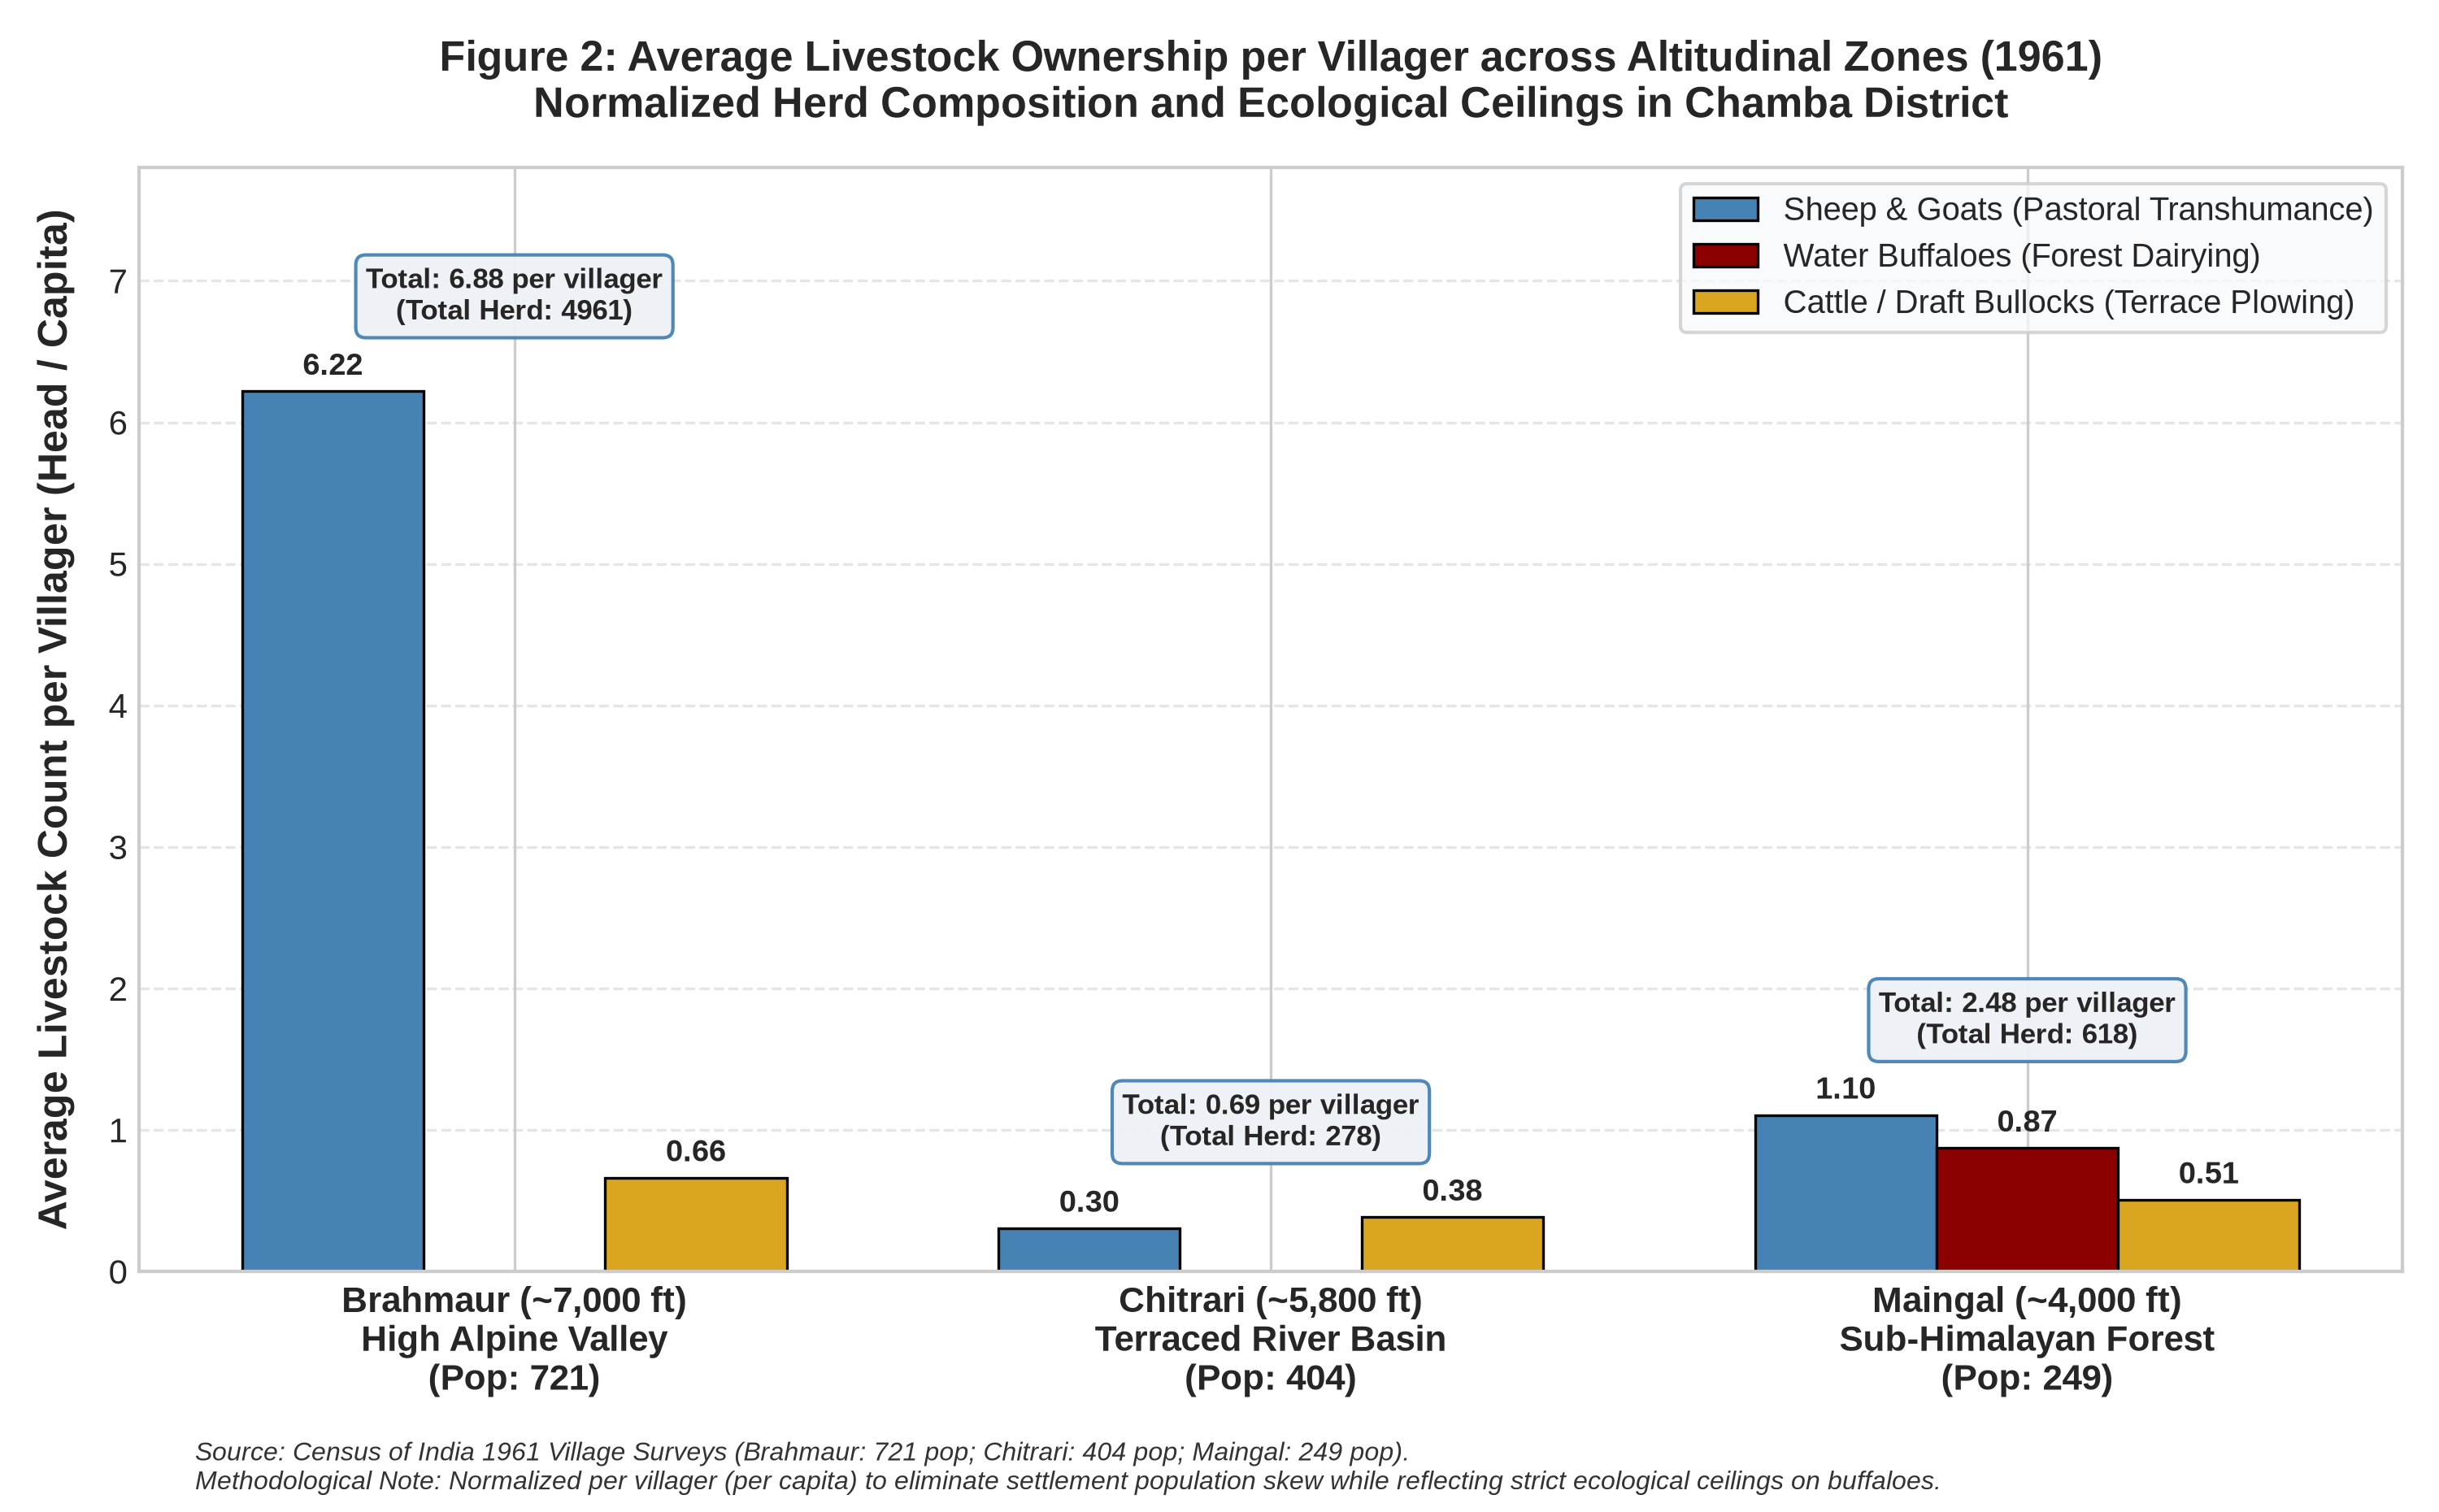
\includegraphics[width=0.88\textwidth]{outputs/figures/fig2_livestock_ecological_distribution.png}
\caption{Livestock Herd Composition across Micro-Ecological Zones (1961). Transhumant sheep/goats concentrate in alpine Brahmaur, draft oxen for terraced tillage in Chitrari, and dairy buffaloes in forested Maingal.}
\label{fig:livestock}
\end{figure}

\section{Labour, Hierarchy, and Economic Interdependence}

Applying Historical Materialism to the village monographs reveals that social hierarchy was not maintained through ceremonial consensus, but through unequal, highly specialized divisions of labour. Dominant landed and pastoral groups who owned accumulated surplus (dead labour) were structurally dependent on subordinate artisan and service communities for living labour power.

\subsection{Brahmaur: The Sipi Tripartite Monopoly}
In alpine Brahmaur, upper-caste Rajputs (40.6\% of population) and Brahmans (34.8\%) owned 97.9\% of the village sheep and goat herds. However, because upper-caste families were occupied with agricultural terraces or ritual duties, they could not manage transhumant migration, shearing, and weaving alone. Sipis (15 households, 119 persons, comprising 16.5\% of the population) occupied an indispensable tripartite monopoly:
\begin{enumerate}[leftmargin=*]
    \item \textbf{Contractual Wage Shepherding (\textit{Pohal}):} Wealthy flock masters hired Sipi men as professional shepherds (\textit{pohals}) to drive thousands of animals across the treacherous glaciated passes of the Dhaula Dhar into Kangra and Lahaul. The Brahmaur monograph (p. 44) details the exact terms of these labour contracts: the \textit{pohal} received free daily meals, coarse clothing, raw wool for his family, a fixed cash wage of Rs. 2/- per month, and an annual dividend of 2 to 4 percent of all newborn lambs. This lamb dividend was a vital material incentive: it aligned the hired shepherd's financial survival with flock reproduction, ensuring diligent protection of pregnant ewes and lambs during blizzards and predator attacks. Here, living wage labour directly mediated the reproduction of pastoral capital.
    \item \textbf{Textile Craftsmanship and Tool Use:} Mountain survival required heavy woollen clothing. Raw fleece sheared thrice yearly (yielding 1 to 1.5 seers per sheep) was processed exclusively by Sipis. Using specialized iron shears (\textit{katar}), carding bows, and horizontal frame pit-looms (\textit{rachh}), Sipis wove durable woolen tweed (\textit{pattu}) and blankets (\textit{gardu}), tailoring the iconic Gaddi flared coat (\textit{chola}) and black sheep's-wool rope sash (\textit{dora}). Upper-caste pastoralists controlled the livestock, but lower-caste craftsmen held the technical means of production required to turn fleece into protective apparel.
    \item \textbf{Ritual Officiation in the Sacred Economy:} In the \textit{Nawala} festival-the central Gaddi sacrificial ceremony dedicated to Lord Shiva-Sipi musicians were indispensable. Throughout an entire night of devotion, Sipi drummers beat the ceremonial \textit{dholak} and chanted sacred verses. In return, they received customary ritual entitlements: grain, cooked food, and the sacred neck of the sacrificed ram (\textit{ghardi}) (Brahmaur Survey, p. 62). Ritual practice thus affirmed both social hierarchy and lower-caste indispensability.
\end{enumerate}

\subsection{Chitrari: Attached Tenancy and Status Contestation}
In Chitrari, where Brahmin households comprised 77.0\% of the population, landed wealth was rooted in centuries-old royal land endowments (\textit{shasan}) attached to the eighth-century Shakti Devi temple. Because Brahmin purity codes strictly forbade touching the wooden stilt of the plough, high-caste proprietors were paralyzed without ploughmen. This labour was supplied by attached \textbf{Halis} (ploughmen). Halis were hereditary tenants who tilled Brahmin lands under tied sharecropping arrangements. 

However, Chitrari documents significant ideological resistance. Embracing the reformist Arya Samaj movement, Halis adopted the official title \textbf{Aryas--Halis} in the 1961 survey (pp. 11--12). By asserting clean Aryan status, they sought to overturn hereditary untouchability and claim social dignity, even as their material livelihoods remained bound to Brahmin landholdings. This tension illustrates the Marxist principle that ideological struggles reflect and contest underlying relations of production.

\subsection{Maingal: Jajmani Blacksmith Barter}
In Maingal, two households of \textbf{Lohar} blacksmiths (8 persons) maintained permanent workshops in Dapaythagot hamlet. They manufactured and sharpened iron ploughshares, sickles, billhooks, and axes for both Muslim Gujjar graziers and Hindu cultivators. Rather than transacting in cash, Lohars were compensated through \textbf{khalian}-customary bundles of unhusked wheat and maize delivered directly from the harvest threshing floors (\textit{khala}) at each agricultural season (Maingal Survey, pp. 38, 40). This custom demonstrates the persistence of non-monetary jajmani exchange alongside commercial markets.

\subsection{Systematic Register of Documented Exchange Relationships}
To formalize these diverse socio-economic interactions across space and time, we compiled a verified register of 12 distinct economic exchange links (Table~\ref{tab:network} and Figure~\ref{fig:network}).

\begin{table}[htbp]
\centering
\footnotesize
\caption{Verified Register of Documented Socio-Economic Exchange Relationships}
\label{tab:network}
\begin{tabularx}{\textwidth}{llp{2.8cm}p{3.2cm}X}
\toprule
\textbf{ID} & \textbf{Spatial Scope} & \textbf{Actor A $\leftrightarrow$ Actor B} & \textbf{Exchange Medium} & \textbf{Historical \& Theoretical Significance} \\
\midrule
R-01 & Brahmaur (Village) & Flock Owner $\leftrightarrow$ Hired Shepherd (\textit{Pohal}) & Cash (Rs. 2/mo), meals, wool, 2--4\% lamb shares & Stratified contractual wage labour emerging within transhumant pastoralism (p. 44). \\
R-02 & Brahmaur (Village) & Flock Owner $\leftrightarrow$ Sipi Weaver/Tailor & Raw wool shares, food grains, meals & Lower-caste technical monopoly over textile manufacturing and shearing (p. 38). \\
R-03 & Brahmaur (Village) & Brahman Priest $\leftrightarrow$ Sipi Musician & Sacrificed sheep neck (\textit{ghardi}), grain & Ritual reciprocity crossing purity/pollution boundaries during \textit{Nawala} feasts (p. 62). \\
R-04 & Brahmaur (Village) & Gaddi Shepherds $\leftrightarrow$ Terraced Cultivators & Overnight sheep penning (\textit{tarkals}) for manure & Agro-pastoral nutrient cycle transferring alpine nitrogen to terraced fields (pp. 45-46). \\
R-05 & Chitrari (Village) & Brahmin Landowner $\leftrightarrow$ Hali Ploughman & Tied crop-share tenancy, land access & Attached ploughing labour circumventing Brahmin taboos; Arya Samaj status contest (p. 11). \\
R-06 & Chitrari (Village) & Hindu Villagers $\leftrightarrow$ Nomadic Gujjars & Cash/grain purchase of milk on high \textit{dhars} & Seasonal inter-community trade supplying essential high-fat dairy nutrition (p. 45). \\
R-07 & Chitrari (Village) & Shakti Temple $\leftrightarrow$ Bensi Pipers & Customary grain perquisites \& temple stipend & Hereditary temple service caste operating within the sacred village economy (p. 32). \\
R-08 & Maingal (Village) & Cultivators $\leftrightarrow$ Lohar Blacksmiths & Customary unhusked grain sheaves (\textit{khalian}) & Customary non-monetary jajmani tool maintenance from harvest threshing floor (p. 33). \\
R-09 & Maingal (Village) & Muslim Gujjars $\leftrightarrow$ Town Bazaar Traders & Cash currency and credit advances for \textit{ghee} & Integration of pastoral dairy surplus into regional cash commodity markets (p. 14). \\
R-10 & Maingal (Village) & Muslim Gujjars $\leftrightarrow$ Hindu Brahmins & Buffalo manure, draft bullock loans, water rights & Peaceful inter-religious co-existence anchored in non-competing ecological niches (p. 12). \\
R-11 & Regional (1881) & Gaddi Herders $\leftrightarrow$ Dual Territorial States & Pasture dues (Chamba) vs. winter land tax (Kangra) & Trans-Dhaula Dhar mobility navigating overlapping sovereign jurisdictions (para 498). \\
R-12 & Regional (1961) & Peasant Families $\leftrightarrow$ Rehara Silversmiths & Cash fee per tola silver crafted + scrap retention & Craft conversion of volatile pastoral livestock profits into portable dowry savings (p. 24). \\
\bottomrule
\end{tabularx}
\end{table}

\begin{figure}[htbp]
\centering
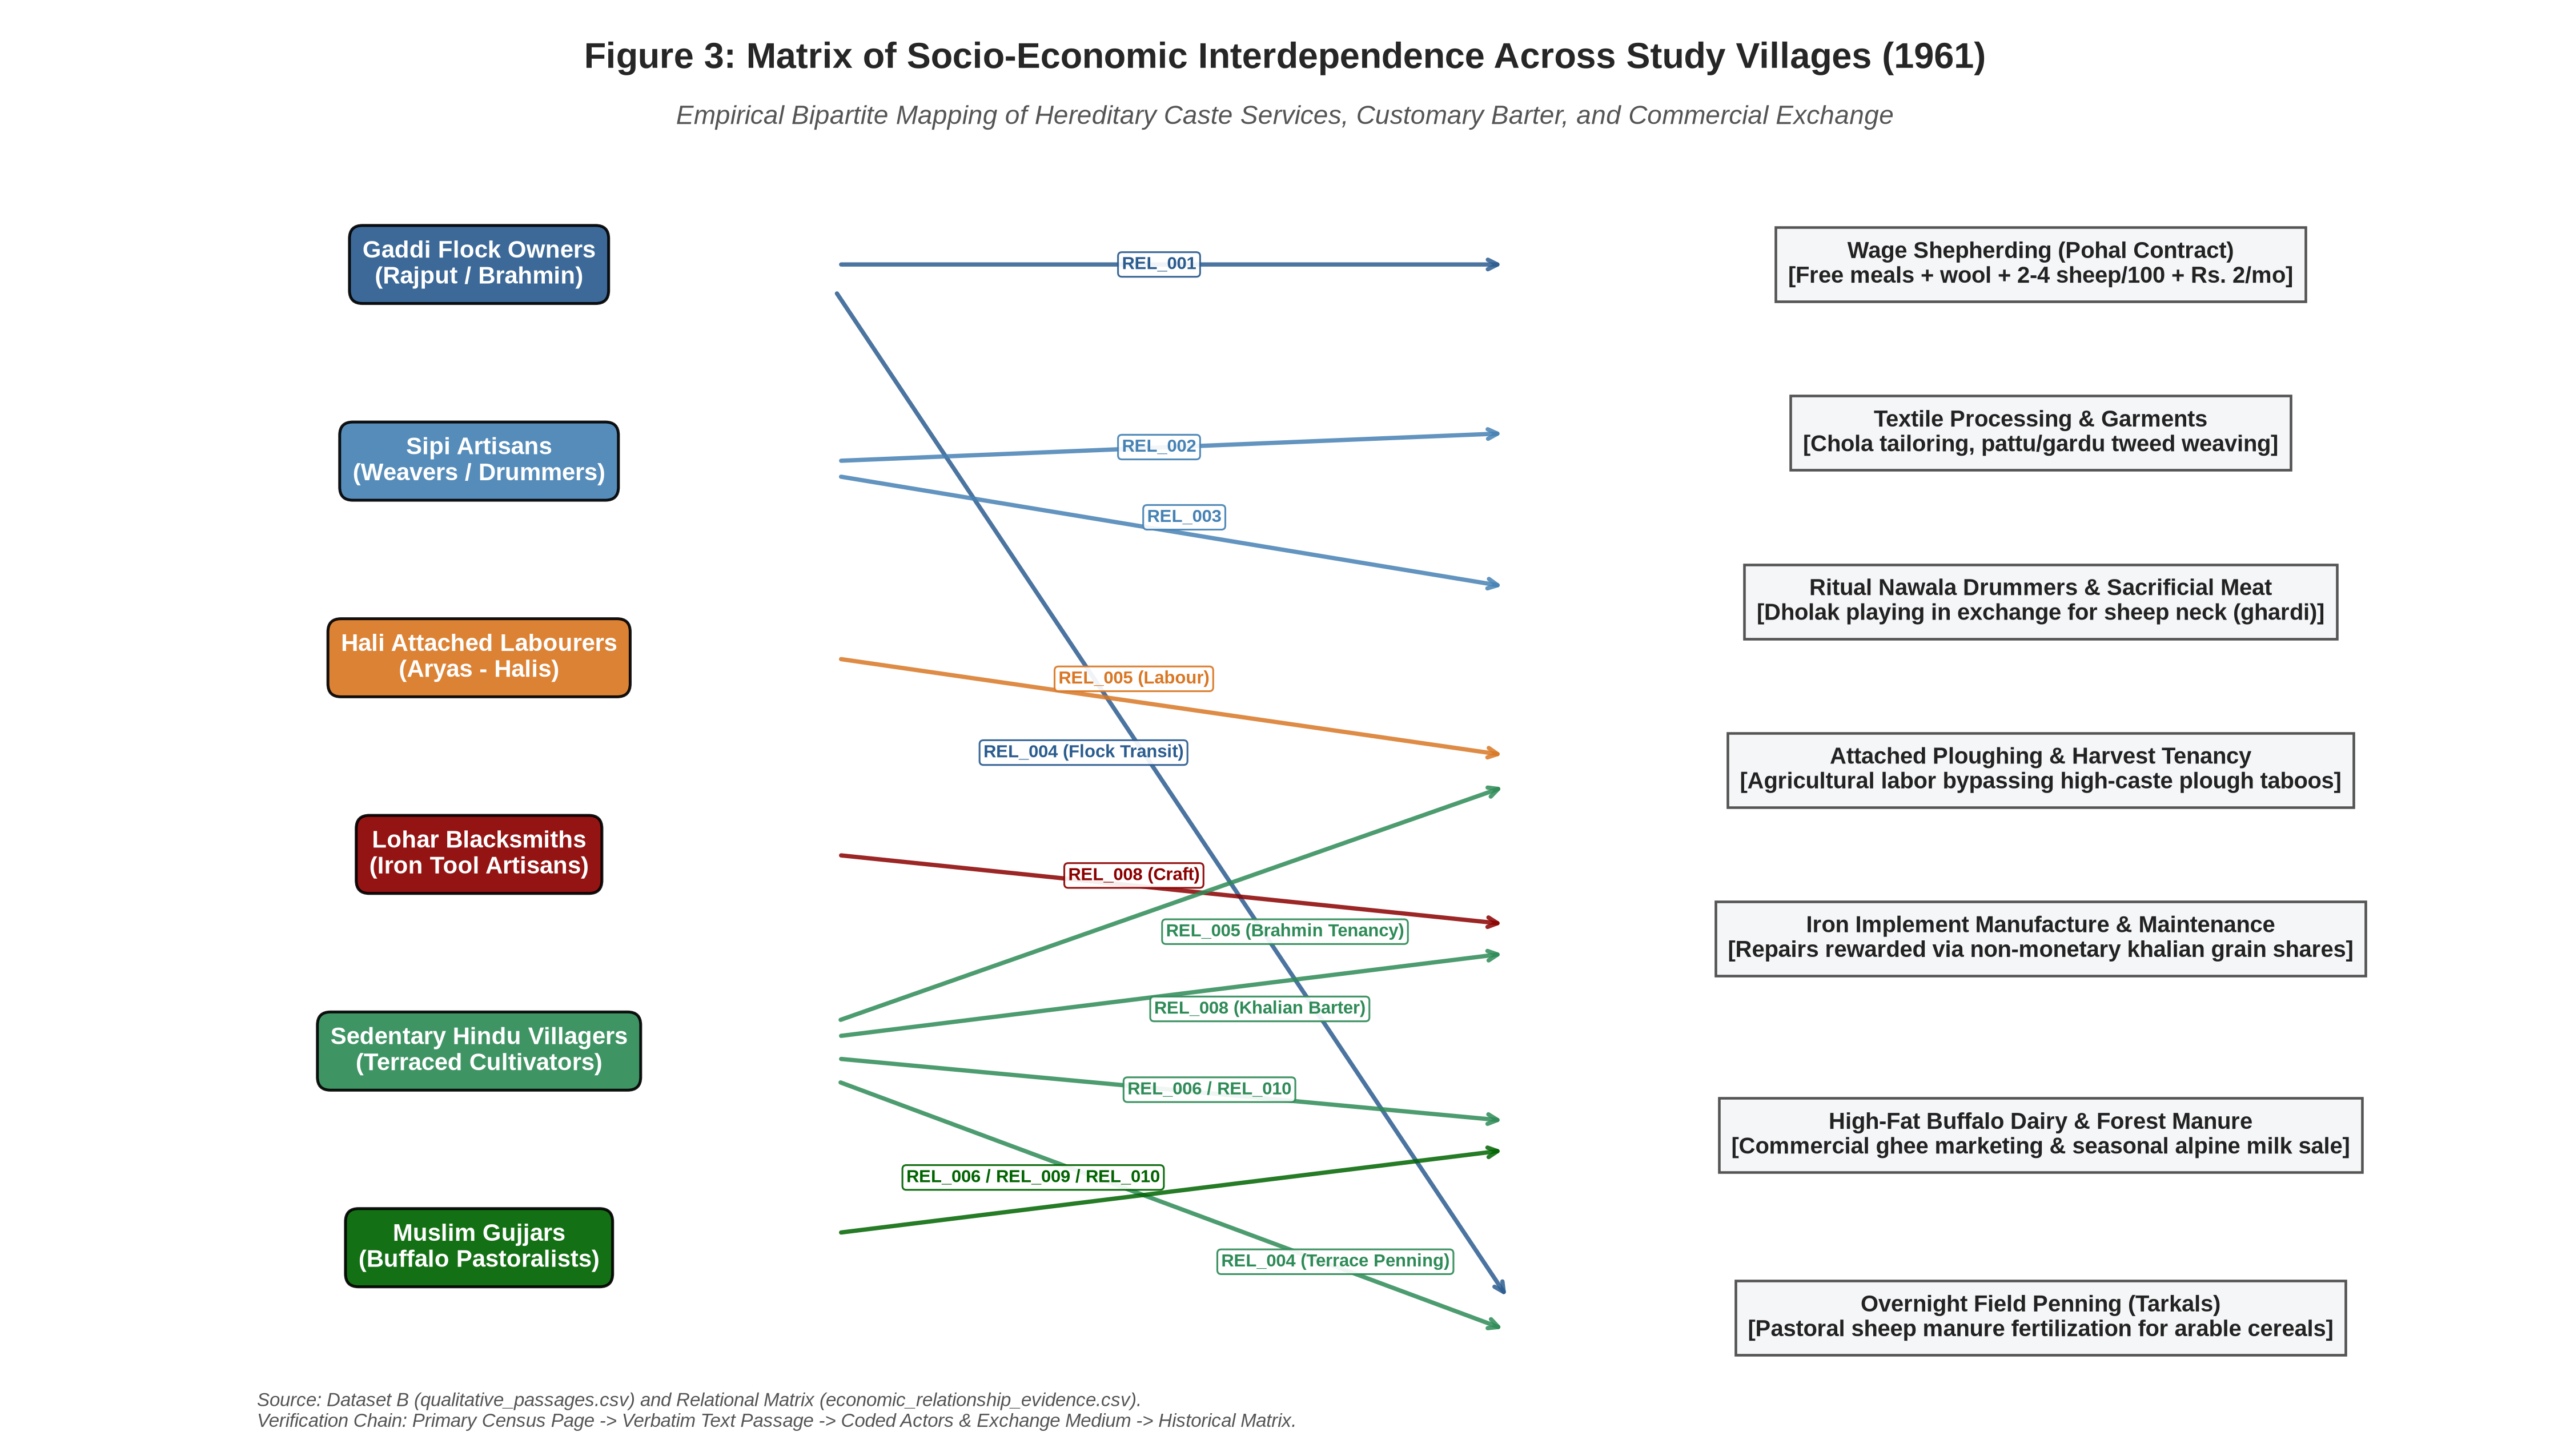
\includegraphics[width=0.92\textwidth]{outputs/figures/fig3_bipartite_economic_exchange.png}
\caption{Bipartite Interaction Matrix Mapping Documented Socio-Economic Interdependence (1961). Nodes represent caste/religious groups and exchange media; edges represent explicit textual proof in the survey monographs.}
\label{fig:network}
\end{figure}

The bipartite network in Figure~\ref{fig:network} illustrates the multi-tiered nature of rural Himalayan exchange. Economic interaction was neither entirely commercial nor wholly customary. Instead, exchange media were stratified: cash contracts governed specialized shepherd labour and bazaar butter sales; customary crop shares supported attached ploughmen and temple pipers; direct in-kind barter maintained village iron tools; and sacrificial meat distributions sustained religious rituals.

\section{Markets, Mobility, and Religious Relations}

A central inquiry of our historical problem concerns how economic organization shaped religious relations. In popular historiography, Hindu-Muslim relations in partitioned northern India are often assumed to have been defined by communal conflict. Rural Chamba presents a distinct historical trajectory.

\subsection{Inter-Religious Co-Existence in Maingal: Complementary Ecological Niches}
In Maingal, 203 Muslim Gujjars (81.5\% of the population across 25 households) lived in peaceful co-residence alongside 34 Hindu Brahmins and 4 Rajputs. Computational coding of qualitative passages reveals that religious harmony was sustained by \textbf{material economic complementarity}:
\begin{itemize}[leftmargin=*]
    \item \textbf{Non-Competing Production Niches:} Muslim Gujjars occupied the forested hill slopes, residing in 13 dispersed hamlets composed of combined dwelling-byre \textit{kothas}. They pastured 217 water buffaloes on forest browse. In contrast, Hindu Brahmins lived in a nucleated settlement in Maingal proper, cultivating terraced maize and wheat plots and operating a water mill (\textit{gharat}) on the Sila stream.
    \item \textbf{Mutual Resource Exchanges:} The two groups exchanged vital productive inputs: Gujjars supplied rich buffalo dung manure to fertilize Brahmin terraced fields, while Brahmin cultivators loaned draft bullocks to Gujjars during seasonal ploughing. The survey explicitly notes the complete absence of communal disputes over land or water (Maingal Survey, pp. 12, 33).
    \item \textbf{Commercial Bazaar Marketing:} Gujjar dairy production was fully commercialized. Women churned buffalo milk into clarified butter (\textit{ghee}), which men transported down the mountain trails to the Chamba town bazaar, selling it for cash or securing credit advances against future deliveries (Maingal Survey, p. 14).
\end{itemize}

\subsection{Chitrari: High-Altitude Seasonal Exchange}
In Chitrari, where 0 Muslims resided permanently, inter-religious contact was organized through \textbf{seasonal, high-altitude market exchange}. Local cows yielded negligible milk (hardly 4--8 chhataks per day). Villagers relied entirely on nomadic Muslim Gujjars camping on high alpine ridges (\textit{dhars}) during the monsoon to purchase milk and butter for cash or grain barter (Chitrari Survey, p. 45).

\subsection{Material Culture as Technological Anchors of Work: Annales Histoire Totale}
Following the \textit{Annales} commitment to total history, material artifacts documented in the village surveys embodied the technological adaptation of human labour to steep mountain ecology:
\begin{enumerate}[leftmargin=*]
    \item \textbf{The Lightweight Wooden Plough (\textit{Hal}) and Iron Socket:} Crafted from oak or wild pear wood, the mountain plough weighed under 15 pounds, allowing a single farmer to carry it across precarious terrace ledges. Socketed with an iron share forged by local Lohars, it physically materialized the caste division of labour: upper-caste Brahmins held the land but were ritually barred from gripping the stilt, making attached Halis indispensable.
    \item \textbf{The Conical Bamboo Basket (\textit{Kilta}):} Fitted with tumpline headstraps, the \textit{kilta} was the universal transport technology of hill women, carrying heavy loads of wet manure (weighing up to 50 pounds) up 45-degree terraced slopes to maintain field fertility.
    \item \textbf{The Dwelling-Byre \textit{Kotha} and Watchtower \textit{Machan}:} In Gujjar hamlets, low flat-roofed stone-timber \textit{kothas} housed families directly above or adjacent to buffalo stalls, utilizing animal body heat to withstand winter freezes. In surrounding fields, farmers erected elevated stilt platforms (\textit{machans}) where men guarded ripening maize against nocturnal bears and wild boars.
    \item \textbf{Portable Silver Dowry Jewelry (\textit{Stridhana}):} Crafted by Reharas, heavy silver ornaments (\textit{chiri}, \textit{ralu}, \textit{kanbali}) allowed transhumant families to convert volatile livestock profits into non-perishable, highly portable savings.
\end{enumerate}

\subsection{Vernacular Oral Evidence: The Emotional Archive of Labour and Mentalit\'es}
Devanagari folk verses mined from the monographs provide indigenous perspectives counterbalancing administrative prose, offering access to subaltern \textit{mentalit\'es}:
\begin{itemize}[leftmargin=*]
    \item \textbf{Women's Transhumant Separation (Chitrari, pp. 72--73):} Sung by Gaddi women left behind during seasonal migration:
    \begin{quote}
    \textit{``Nange pairin main dhar chadhi jaandi...''} [Barefoot I climb the thorny alpine ridge...]
    \end{quote}
    The verses articulate the intense physical torment of highland ascent, the burden of managing household cultivation alone, and structural dependence on the village revenue accountant (\textit{Patwari}) to read and write letters across the snow passes.
    \item \textbf{The Sacrificial Vow (\textit{Shiv Ainchali}, Brahmaur, p. 66):} Records the sacrificial offering of 84 sheep to Lord Shiva, documenting how Brahmins, spirit mediums (\textit{chelas}), and Sipi drummers assembled across caste lines to consume sanctified meat.
    \item \textbf{Shepherd's Death in a Blizzard (\textit{Bhohku Git}, Brahmaur, p. 58):} Mourns the death of shepherd Bhukhu frozen in an unseasonal blizzard on the high mountain pass (\textit{jot}), relaying news of his lost flock through trans-Himalayan Lahauli caravaneers.
\end{itemize}

\section{Historical Change and Colonial Categories (1881--1961)}

To trace socio-economic transformation over eighty years without committing anachronism, we must examine how state classification systems evolved. The categories recorded by census enumerators were not neutral mirrors of reality, but situated colonial interventions that shaped how society was seen and governed (Table~\ref{tab:crosswalk}).

\begin{table}[htbp]
\centering
\footnotesize
\setlength{\tabcolsep}{4pt}
\caption{Multi-Temporal Historical Classification Crosswalk (1881--1961)}
\label{tab:crosswalk}
\begin{tabularx}{\textwidth}{llp{2.8cm}X}
\toprule
\textbf{Category} & \textbf{Historical Era \& Source} & \textbf{Original Term in Text} & \textbf{Classification Logic \& Historiographical Caveat} \\
\midrule
\textbf{Gaddi} & 1881 Census (Ibbetson) & \textit{Gadi} (para 498) & Occupational-geographic label; includes Brahmans/Khatris; excludes impure service castes (Sipis, Halis). Paternal revenue lens. \\
& 1911 Glossary (Rose, Vol. II) & \textit{Gaddi} (p. 256) & 4-tier racialized hierarchy; invents Mughal flight myth to explain Khatri presence; essentializes fluid pastoral transhumance. \\
& 1931 Census (Khan, Vol. XVII) & \textit{Gaddi} (p. 285) & Enumerated as Hill Tribe; cross-tabulated with depression economic dependency categories (Earners/Dependents). \\
& 1961 Survey (Monograph No. 5) & \textit{Gaddi} (Scheduled Tribe) & Statutory constitutional category (1956); unifies upper/lower castes under legal umbrella despite persistent internal hierarchy. \\
\midrule
\textbf{Gujjar} & 1881 Census (Ibbetson) & \textit{Gujar} (para 481) & Broad provincial cattle grazier category; bundles plains farmers with transhumant forest buffalo graziers. \\
& 1911 Glossary (Rose, Vol. II) & \textit{Gujar} (p. 308) & Pejorative administrative stereotyping: ``lazy cultivator... fond of other people's cattle.'' Anti-pastoral revenue prejudice. \\
& 1961 Survey (Monograph No. 27) & \textit{Muslim Gujjar} (ST) & Micro-census of settled forest dairy producers; 217 buffaloes; commercial ghee marketing in Chamba bazaar. \\
\midrule
\textbf{Sipi} & 1881 Census (Ibbetson) & \textit{Sipi} (para 498) & Grouped with Badis and Halis as generic impure menials excluded from true Gaddi status. \\
& 1914 Glossary (Rose, Vol. III) & \textit{Sipi / Sippi} (p. 407) & Defined specifically as professional sheep-shearers and weavers in Barmaur wizarat; servile framing. \\
& 1961 Survey (Monograph No. 5) & \textit{Sipi} (Scheduled Caste) & Documents tripartite monopoly: contracted wage-shepherds (\textit{pohals}), tweed weavers, and \textit{Nawala} ritual drummers. \\
\midrule
\textbf{Hali} & 1881 Census (Ibbetson) & \textit{Hali} (para 498) & Functional ploughman category derived from \textit{hal} (plough); classified as impure service group. \\
& 1911 Glossary (Rose, Vol. II) & \textit{Hali} (p. 324) & Hereditary attached serfs performing ploughing for landowners under high-caste plough taboos. \\
& 1961 Survey (Monograph No. 10) & \textit{Aryas--Halis} (SC) & Hyphenated title capturing active Arya Samaj mobilization against untouchability while remaining attached ploughmen. \\
\bottomrule
\end{tabularx}
\end{table}

\subsection{Categorical Drift vs. Real Socio-Economic Transformation}
Analyzing the historical crosswalk illuminates how administrative reclassification often masked underlying economic continuities:
\begin{enumerate}[leftmargin=*]
    \item \textbf{From Racial Ethnography to Economic Dependency:} In 1881 and 1911, the colonial state categorized hill populations through hereditary caste and racial stereotypes. By 1931, confronting the dislocation of the Great Depression, the colonial census abandoned caste-based vocational tables in favor of modern functional categories: \textbf{Principal Earners}, \textbf{Working Dependents}, and \textbf{Non-Working Dependents} (Khan 1933, Vol. XVII, pp. 210--215). In Chamba State, the census recorded 30,665 occupied houses across a rural population of 146,870 (yielding an average household density of 4.79 persons per house). This transition reflected the state's urgent need to assess agrarian depression and tax-bearing capacity, rather than a disappearance of caste-based labour.
    \item \textbf{Colonial Class Alliance and Revenue Extraction:} In Marxist historiography, colonialism is understood as a systemic mode of extraction transferring resources from periphery to metropolis, dividing both colonizer and colonized along class lines. In Chamba, the British Crown maintained indirect rule through the princely Raja, creating a class alliance between colonial authorities and native feudal rulers that preserved traditional agrarian extractions while imposing commercial timber and pasture regulations.
    \item \textbf{Statutory Homogenization vs. Internal Hierarchy:} In 1956, the Government of India designated ``Gaddi'' as a Scheduled Tribe. In administrative discourse, this statutory label unified all inhabitants of Brahmaur under a common indigenous identity. However, as our 1961 micro-data demonstrates, internal caste stratifications persisted intact: upper-caste Rajputs owned the flocks, while lower-caste Sipis remained wage-earning shepherds, weavers, and ritual drummers.
    \item \textbf{Genuine Subaltern Mobilization:} The emergence of the term \textit{Aryas--Halis} in Chitrari was not a top-down bureaucratic invention, but bottom-up agency. Attached ploughmen utilized the egalitarian ideology of the Arya Samaj to demand ritual dignity, even as their material dependence on Brahmin land remained unsevered.
\end{enumerate}

\section{Conclusion}

This study has investigated how changing patterns of occupation and economic interdependence shaped caste and religious relations in Brahmaur, Chitrari, and Maingal of Chamba District from 1881 to 1961. Synthesizing Historical Materialism and the \textit{Annales} school with computational text mining, concordance parsing, network analysis, and qualitative thematic coding, our findings provide a definitive answer to the historical problem:
\begin{enumerate}[leftmargin=*]
    \item \textbf{Environmental Altitudes Imposed Absolute Biological Ceilings (\textit{Longue Dur\'ee}):} Mountain relief established strict physiological boundaries on pastoral husbandry. Water buffaloes suffered catastrophic lactation collapse (dropping from 9 to 4 seers per day) when introduced to alpine Brahmaur ($\sim$7,000 ft), permanently barring them from high elevations and reserving commercial dairy production for sub-Himalayan Maingal ($\sim$4,000 ft). This ecological ceiling secured the Gaddi monopoly over alpine transhumant sheep pastoralism and created an exclusive niche for Gujjar forest dairying.
    \item \textbf{Asymmetrical Labour Divisions Sustained Caste Hierarchy (\textit{Dead vs. Living Labour}):} Himalayan villages were not autarkic republics, but tightly integrated moral economies. Dominant Rajput and Brahmin proprietors who controlled accumulated surplus (dead labour in land and flocks) were structurally dependent on subordinate living labour: Sipis in Brahmaur monopolized wage shepherding, cloth weaving, and ritual music; attached Halis in Chitrari performed essential ploughing to circumvent high-caste purity taboos; and Lohars in Maingal maintained agricultural iron tools in exchange for customary unhusked grain sheaves (\textit{khalian}).
    \item \textbf{Persistence of Multi-Tiered Economic Systems (\textit{Conjuncture}):} The expansion of cash markets did not destroy customary exchange. Instead, contractual cash wages, tied crop-share tenancies, non-monetary jajmani threshing perquisites, and commercial bazaar sales functioned concurrently as a multi-tiered economic system.
    \item \textbf{Religious Co-existence Grounded in Ecological Complementarity:} Peaceful Hindu-Muslim co-residence in Maingal and seasonal trade in Chitrari were anchored in non-competing ecological niches between mobile forest pastoralists and sedentary valley cultivators, who exchanged manure, draft bullocks, water rights, and dairy products without resource conflict.
\end{enumerate}

By combining computational text analysis with close reading of the colonial and post-colonial archive, this study demonstrates that Himalayan societies were neither timeless traditional isolates nor passive victims of modernization, but dynamic communities actively negotiating hierarchy, labour, and survival within the formidable structures of the high mountains.

\section*{Archival and Primary Source References}
\begin{enumerate}[leftmargin=*]
    \item Ibbetson, Denzil Charles Jelf. \textit{Report on the Census of the Panj\'ab Taken on the 17th of February 1881}. 6 vols. Calcutta: Central Press, 1883.
    \item Rose, Horace Arthur. \textit{A Glossary of the Tribes and Castes of the Punjab and North-West Frontier Province}. Based on the Census Reports of Denzil Ibbetson (1881) and Edward Maclagan (1891). 3 vols. Lahore: Samuel T. Weston / Civil and Military Gazette Press, 1911--1919.
    \item Khan, Khan Ahmad Hasan. \textit{Census of India, 1931. Volume XVII: Punjab, Part I-Report}. Lahore: Civil and Military Gazette Press, 1933.
    \item Singh, Ram Chandra Pal, ed. \textit{Census of India 1961. Volume XX, Part VI: Himachal Pradesh-A Village Survey, No. 5: Brahmaur}. Delhi: Manager of Publications, Government of India, 1963.
    \item Singh, Ram Chandra Pal, ed. \textit{Census of India 1961. Volume XX, Part VI: Himachal Pradesh-A Village Survey, No. 10: Chitrari}. Delhi: Manager of Publications, Government of India, 1964.
    \item Singh, Ram Chandra Pal, ed. \textit{Census of India 1961. Volume XX, Part VI: Himachal Pradesh-A Village Survey, No. 27: Maingal}. Delhi: Manager of Publications, Government of India, 1966.
\end{enumerate}

\end{document}